\section{CD\texorpdfstring{$^+$}{+} + He rate coefficients}
\label{appendix:CD+_simulation_rates}

\begin{table}[!htb]
    \centering

    \caption{Derived attachment and dissociation rate coefficients ($k_3\ \&\ k_{CID}$) and rates($R_3\ \&\ R_{CID}$), for \CD molecular ion collision with helium buffer gas at $2.2 \cdot 10^{14}$ cm$^{-3}$ number density. The rates are given for up to two complexes, i.e., He\CD and He$_2$CD$^+$.}
    \label{appendix:tab:attachment-rate-coefficients}
    \begin{tabular}{rll|ll}
        \hline

                  & $k_3$                & $R_3$   & $k_{CID}$            & $R_{CID}$ \\
                  & [\ccpers]            & [\pers] & [\cccpers]           & [\pers]   \\
        \hline\hline                                                                  \\
        He\CD     & $1.1 \cdot 10^{-30}$ & $0.053$ & $5.9 \cdot 10^{-16}$ & $0.130$   \\
        He$_2$\CD & $3.6 \cdot 10^{-30}$ & $0.174$ & $1.2 \cdot 10^{-15}$ & $0.264$   \\
        \hline\hline                                                                  \\
    \end{tabular}
\end{table}

\begin{longtable}[!htb]{rclll}
    % \centering
    \caption{Derived collisional rates at $T=7$ K (derived from \cite{Werfelli2017}), CD$^+$ collision with He [$2.2 \cdot 10^{14}$ cm$^{-3}$ number density] for an initial $|i\rangle$ state transitions into final $|j\rangle$ state via $k_{ij}$ rate coefficients [in cm$^3$/s] and $R_{ij}$ rate [in s$^{-1}$].}
    \label{appendix:tab:collisional-rate-coefficients}                  \\
    % \begin{tabular}{rclll}
    \hline
    i &               & j & $k_{ij}$             & $R_{ij}$             \\
    \hline\hline                                                        \\
    0 & $\rightarrow$ & 1 & $9.9 \cdot 10^{-11}$ & $2.2 \cdot 10^{4}$   \\
    0 & $\rightarrow$ & 2 & $6.3 \cdot 10^{-11}$ & $1.4 \cdot 10^{4}$   \\
    1 & $\rightarrow$ & 2 & $1.6 \cdot 10^{-10}$ & $3.4 \cdot 10^{4}$   \\
    0 & $\rightarrow$ & 3 & $4.3 \cdot 10^{-11}$ & $9.4 \cdot 10^{3}$   \\
    1 & $\rightarrow$ & 3 & $6.1 \cdot 10^{-11}$ & $1.3 \cdot 10^{4}$   \\
    2 & $\rightarrow$ & 3 & $1.5 \cdot 10^{-10}$ & $3.2 \cdot 10^{4}$   \\
    0 & $\rightarrow$ & 4 & $5.5 \cdot 10^{-12}$ & $1.2 \cdot 10^{3}$   \\
    1 & $\rightarrow$ & 4 & $5.8 \cdot 10^{-11}$ & $1.3 \cdot 10^{4}$   \\
    2 & $\rightarrow$ & 4 & $8.7 \cdot 10^{-11}$ & $1.9 \cdot 10^{4}$   \\
    3 & $\rightarrow$ & 4 & $1.3 \cdot 10^{-10}$ & $2.9 \cdot 10^{4}$   \\
    0 & $\rightarrow$ & 5 & $1.4 \cdot 10^{-11}$ & $3.1 \cdot 10^{3}$   \\
    1 & $\rightarrow$ & 5 & $2.0 \cdot 10^{-11}$ & $4.4 \cdot 10^{3}$   \\
    2 & $\rightarrow$ & 5 & $5.7 \cdot 10^{-11}$ & $1.3 \cdot 10^{4}$   \\
    3 & $\rightarrow$ & 5 & $1.0 \cdot 10^{-10}$ & $2.3 \cdot 10^{4}$   \\
    4 & $\rightarrow$ & 5 & $1.2 \cdot 10^{-10}$ & $2.7 \cdot 10^{4}$   \\
    \\
    1 & $\rightarrow$ & 0 & $1.3 \cdot 10^{-11}$ & $2.9 \cdot 10^{3}$   \\
    2 & $\rightarrow$ & 0 & $2.8 \cdot 10^{-14}$ & $6.2 \cdot 10^{0}$   \\
    2 & $\rightarrow$ & 1 & $5.2 \cdot 10^{-13}$ & $1.1 \cdot 10^{2}$   \\
    3 & $\rightarrow$ & 0 & $2.4 \cdot 10^{-18}$ & $5.2 \cdot 10^{-4}$  \\
    3 & $\rightarrow$ & 1 & $2.5 \cdot 10^{-17}$ & $5.6 \cdot 10^{-3}$  \\
    3 & $\rightarrow$ & 2 & $1.8 \cdot 10^{-14}$ & $4.1 \cdot 10^{0}$   \\
    4 & $\rightarrow$ & 0 & $1.6 \cdot 10^{-24}$ & $3.5 \cdot 10^{-10}$ \\
    4 & $\rightarrow$ & 1 & $1.3 \cdot 10^{-22}$ & $2.8 \cdot 10^{-8}$  \\
    4 & $\rightarrow$ & 2 & $5.7 \cdot 10^{-20}$ & $1.3 \cdot 10^{-5}$  \\
    4 & $\rightarrow$ & 3 & $6.8 \cdot 10^{-16}$ & $1.5 \cdot 10^{-1}$  \\
    5 & $\rightarrow$ & 0 & $9.4 \cdot 10^{-31}$ & $2.1 \cdot 10^{-16}$ \\
    5 & $\rightarrow$ & 1 & $9.9 \cdot 10^{-30}$ & $2.2 \cdot 10^{-15}$ \\
    5 & $\rightarrow$ & 2 & $8.4 \cdot 10^{-27}$ & $1.8 \cdot 10^{-12}$ \\
    5 & $\rightarrow$ & 3 & $1.2 \cdot 10^{-22}$ & $2.7 \cdot 10^{-8}$  \\
    5 & $\rightarrow$ & 4 & $2.8 \cdot 10^{-17}$ & $6.1 \cdot 10^{-3}$  \\
    \hline\hline                                                        \\
    % \end{tabular}
\end{longtable}

\begin{table}[!htb]
    \centering
    \caption{Derived radiative rates at P=$3.5 \cdot 10^{-5}$ W, for an initial $|i\rangle$ state transitions into final $|j\rangle$ state with $A_{ij}$ spontaneous emission, $B_{ij}$ stimulated absorption and $B_{ji}$ stimulated emission. The spontaneous emission rates are derived from the effective Hamiltonian fitting of \CD ion using the Pgopher program \cite{western_pgopher_2017}. Subsequently, the stimulated emissions are computed from spontaneous emission rates (see Section \ref{subsec:ROSAA-simulation-rad}). All $A_{ij}$, $B_{ij}$ and $B_{ji}$ are in units of s$^{-1}$.}
    \label{appendix:tab:radiative-rate-coefficients}
    \begin{tabular}{rclll}
        \hline
        i & j & $A_{ij}$            & $B_{ij}$           & $B_{ji}$           \\
        \hline\hline                                                          \\
        1 & 0 & $3.6 \cdot 10^{-4}$ & $2.5 \cdot 10^{4}$ & $7.4 \cdot 10^{4}$ \\
        2 & 1 & $3.5 \cdot 10^{-3}$ & $3.0 \cdot 10^{4}$ & $4.9 \cdot 10^{4}$ \\
        3 & 2 & $1.3 \cdot 10^{-2}$ & $3.2 \cdot 10^{4}$ & $4.4 \cdot 10^{4}$ \\
        4 & 3 & $3.1 \cdot 10^{-2}$ & $3.3 \cdot 10^{4}$ & $4.2 \cdot 10^{4}$ \\
        5 & 4 & $6.1 \cdot 10^{-2}$ & $3.4 \cdot 10^{4}$ & $4.1 \cdot 10^{4}$ \\
        \hline\hline                                                          \\
    \end{tabular}
\end{table}

% \section{N\texorpdfstring{$^+$}\ + He rate coefficients}

\begin{figure}[!htb]
    \centering
    \begin{adjustbox}{minipage=\linewidth,scale=0.8}
    \Subfigure[0.48]{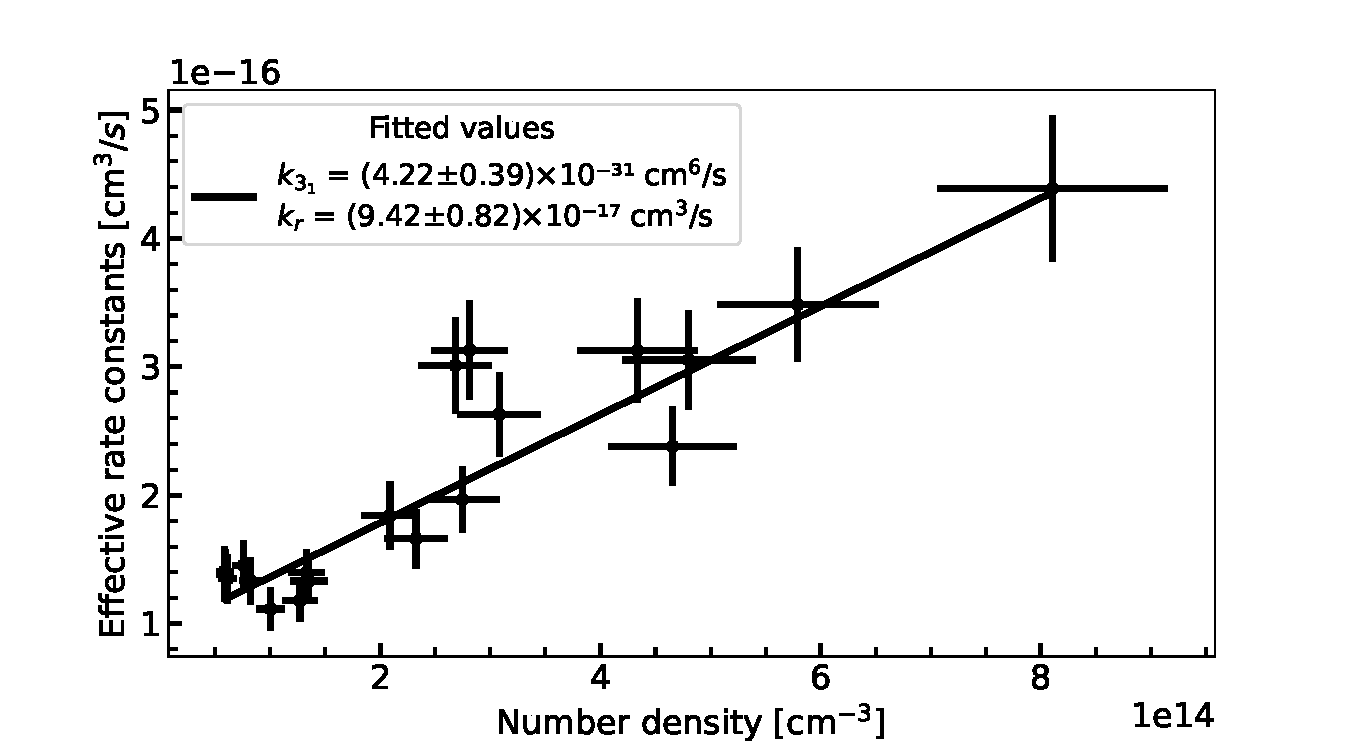
\includegraphics[width=1\textwidth]{figures/measurements/kinetics/functionOf_nHe/N+/off_4.7K_k31_effective_rate_constants.pdf}}{}{\label{fig:off:4.7k-effective-rate-constants:N+}}
    \hfill
    \Subfigure[0.48]{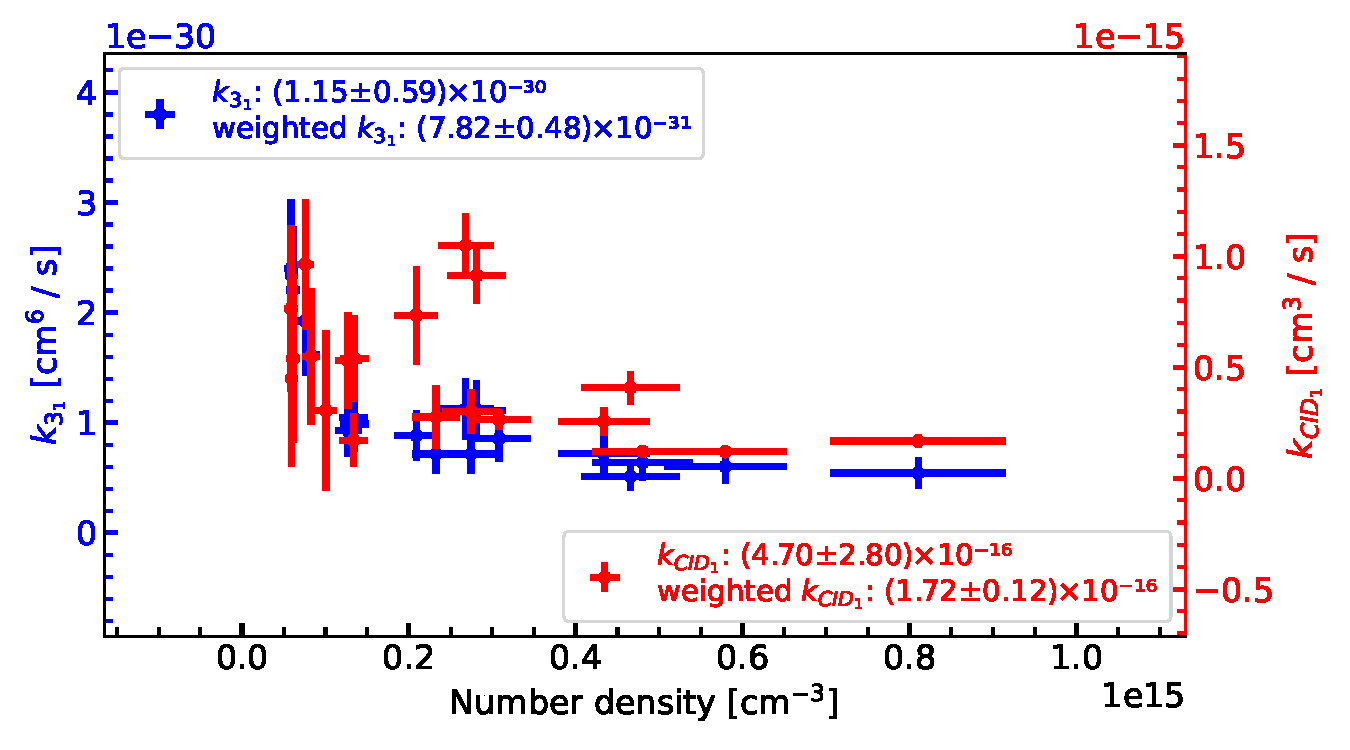
\includegraphics[width=1\textwidth]{figures/measurements/kinetics/functionOf_nHe/N+/off_4.7K_k3_kCID_1_as_functionOfnHe.pdf}}{}{\label{fig:off:4.7k-rate-constants:N+}}
    \hfill
    \Subfigure[0.48]{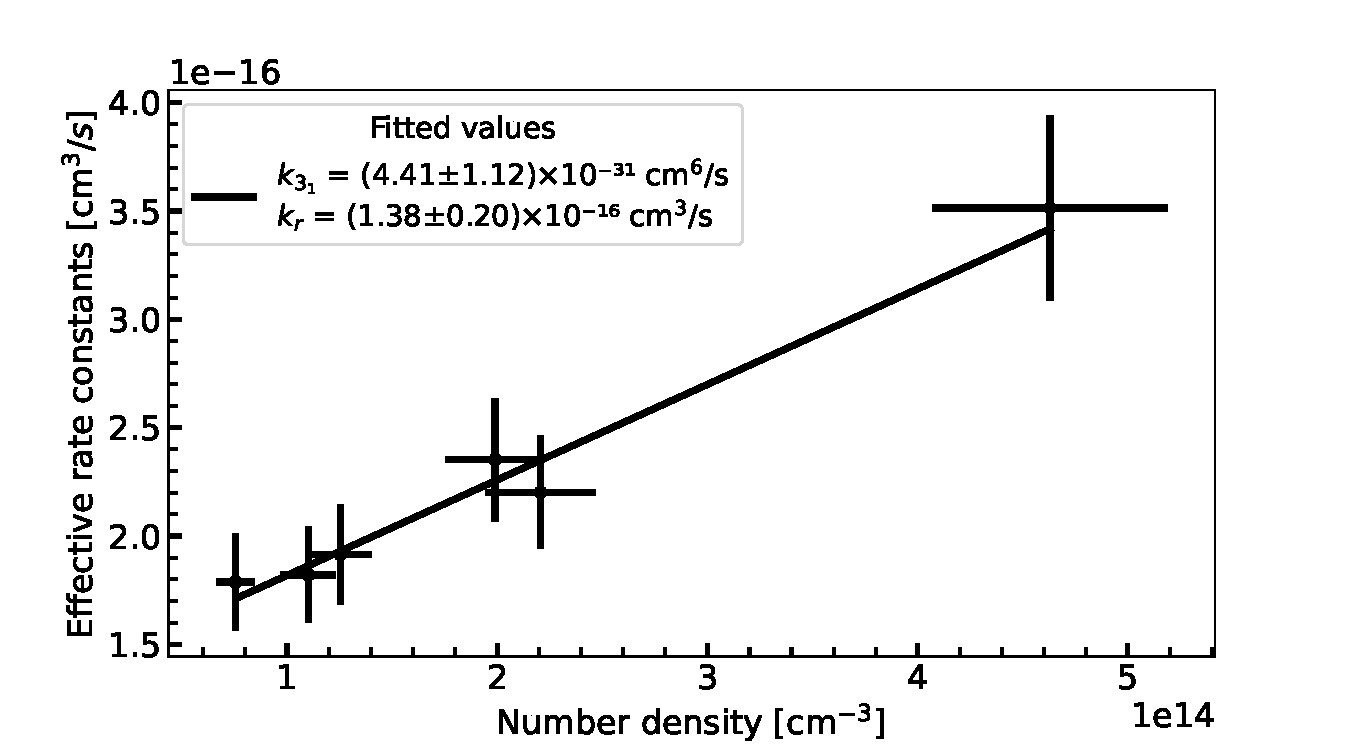
\includegraphics[width=1\textwidth]{figures/measurements/kinetics/functionOf_nHe/N+/off_6.5K_k31_effective_rate_constants.pdf}}{}{\label{fig:off:6.5k-effective-rate-constants:N+}}
    \hfill
    \Subfigure[0.48]{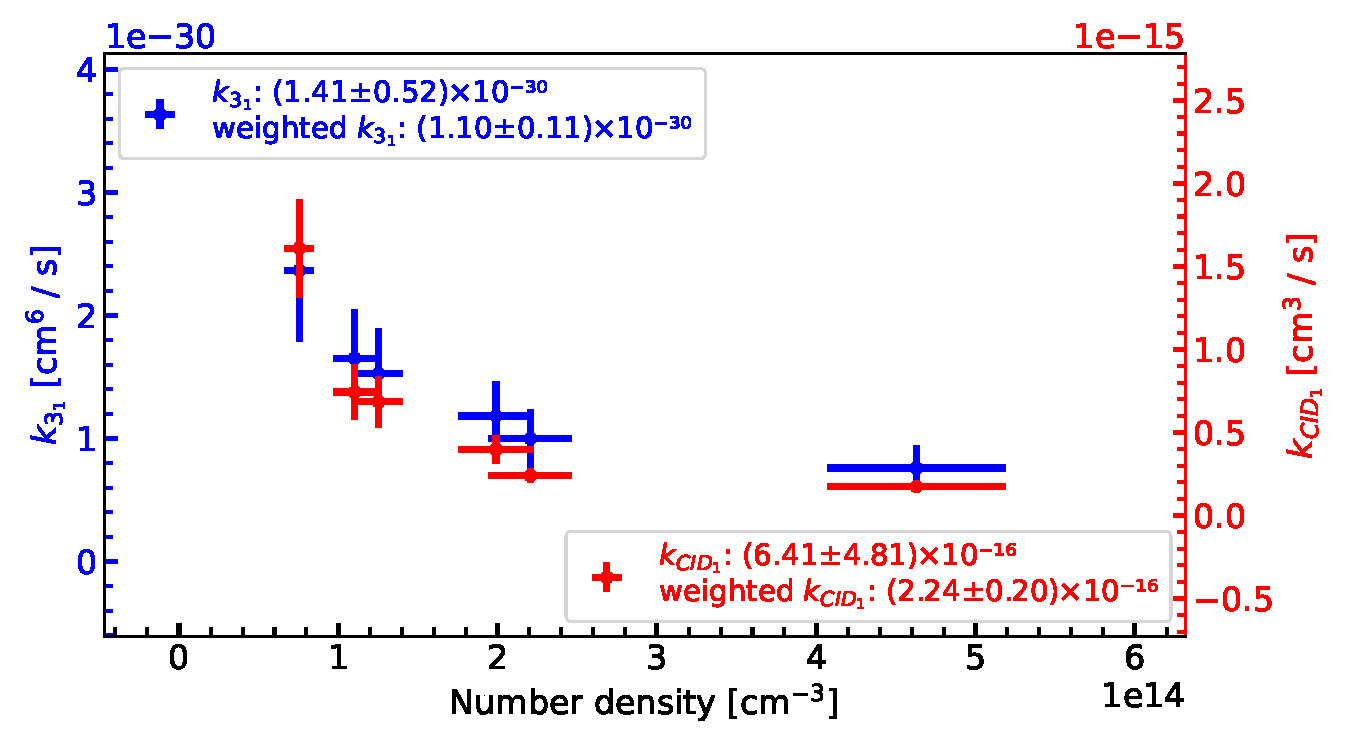
\includegraphics[width=1\textwidth]{figures/measurements/kinetics/functionOf_nHe/N+/off_6.5K_k3_kCID_1_as_functionOfnHe.pdf}}{}{\label{fig:off:6.5k-rate-constants:N+}}
    \hfill
    \Subfigure[0.48]{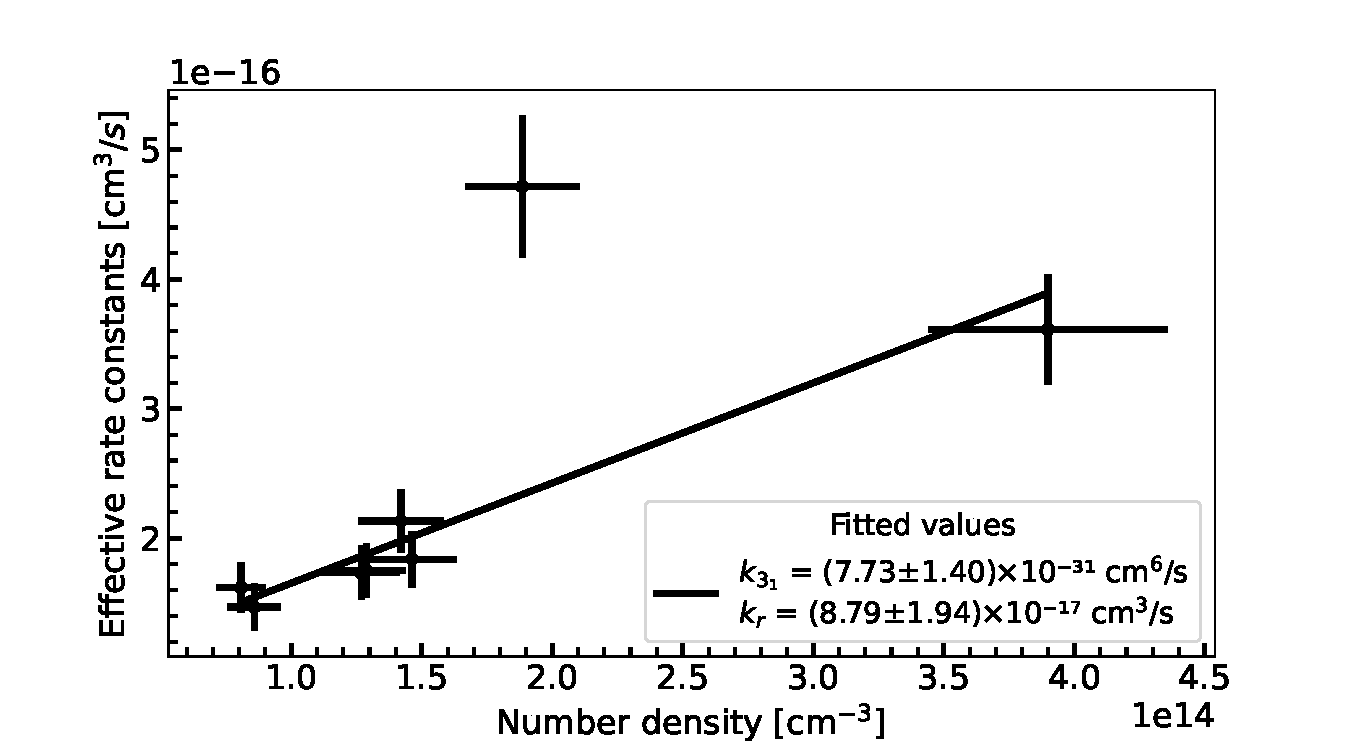
\includegraphics[width=1\textwidth]{figures/measurements/kinetics/functionOf_nHe/N+/off_8.4K_k31_effective_rate_constants.pdf}}{}{\label{fig:off:8.4k-effective-rate-constants:N+}}
    \hfill
    \Subfigure[0.48]{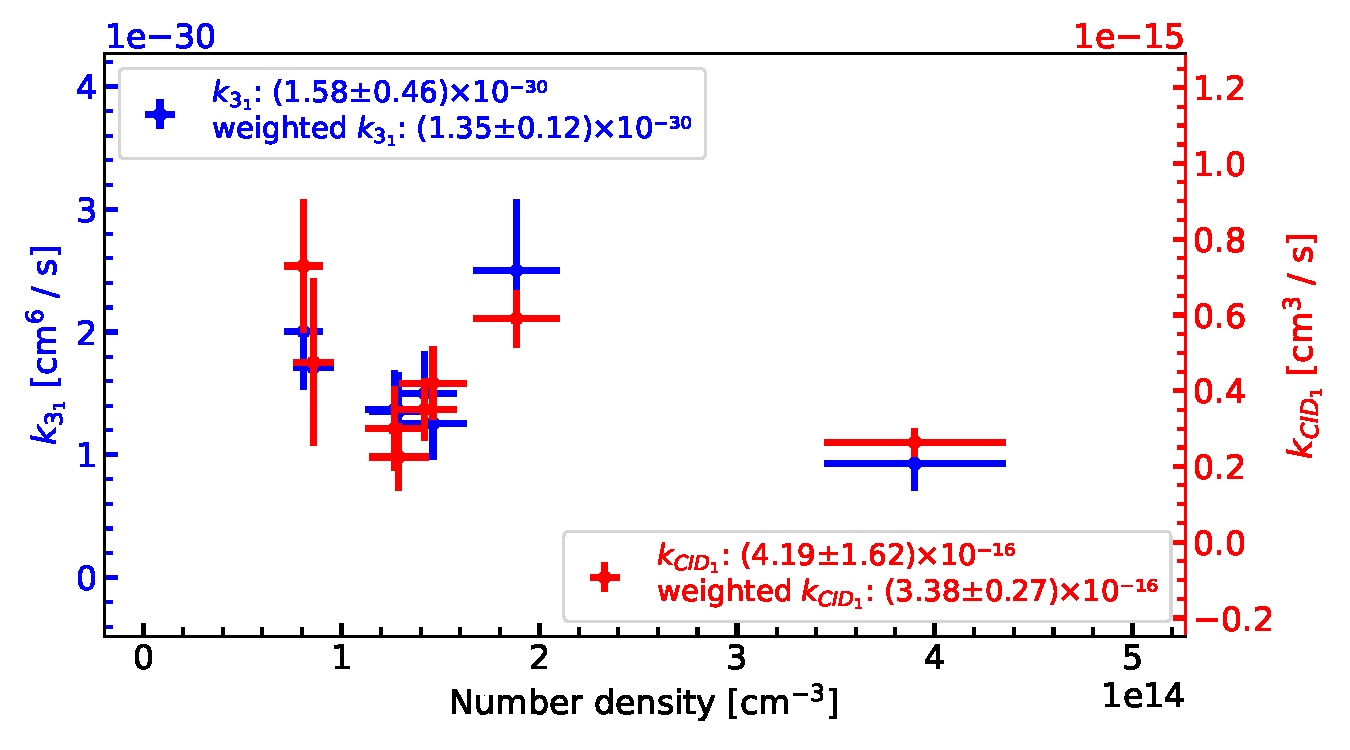
\includegraphics[width=1\textwidth]{figures/measurements/kinetics/functionOf_nHe/N+/off_8.4K_k3_kCID_1_as_functionOfnHe.pdf}}{}{\label{fig:off:8.4k-rate-constants:N+}}
    \hfill
    \Subfigure[0.48]{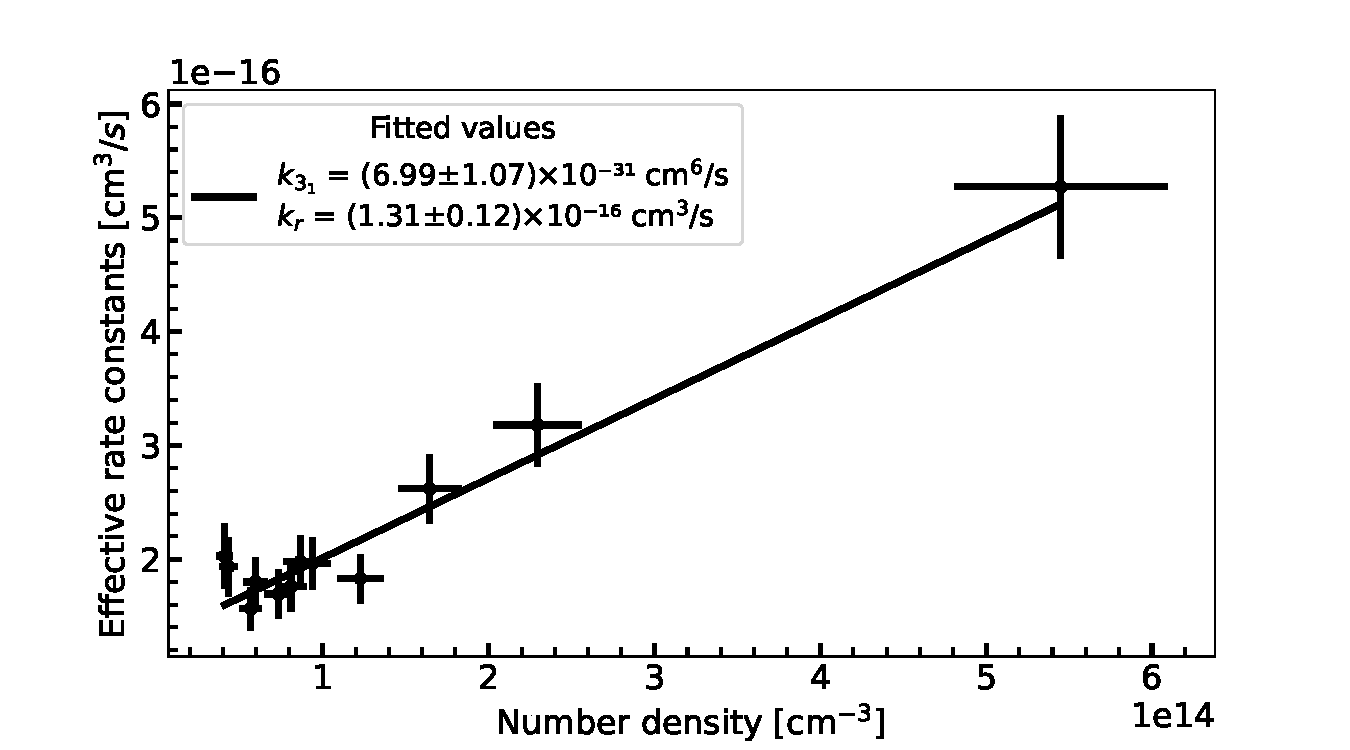
\includegraphics[width=1\textwidth]{figures/measurements/kinetics/functionOf_nHe/N+/off_10K_k31_effective_rate_constants.pdf}}{}{\label{fig:10k-off:effective-rate-constants:N+}}
    \hfill
    \Subfigure[0.48]{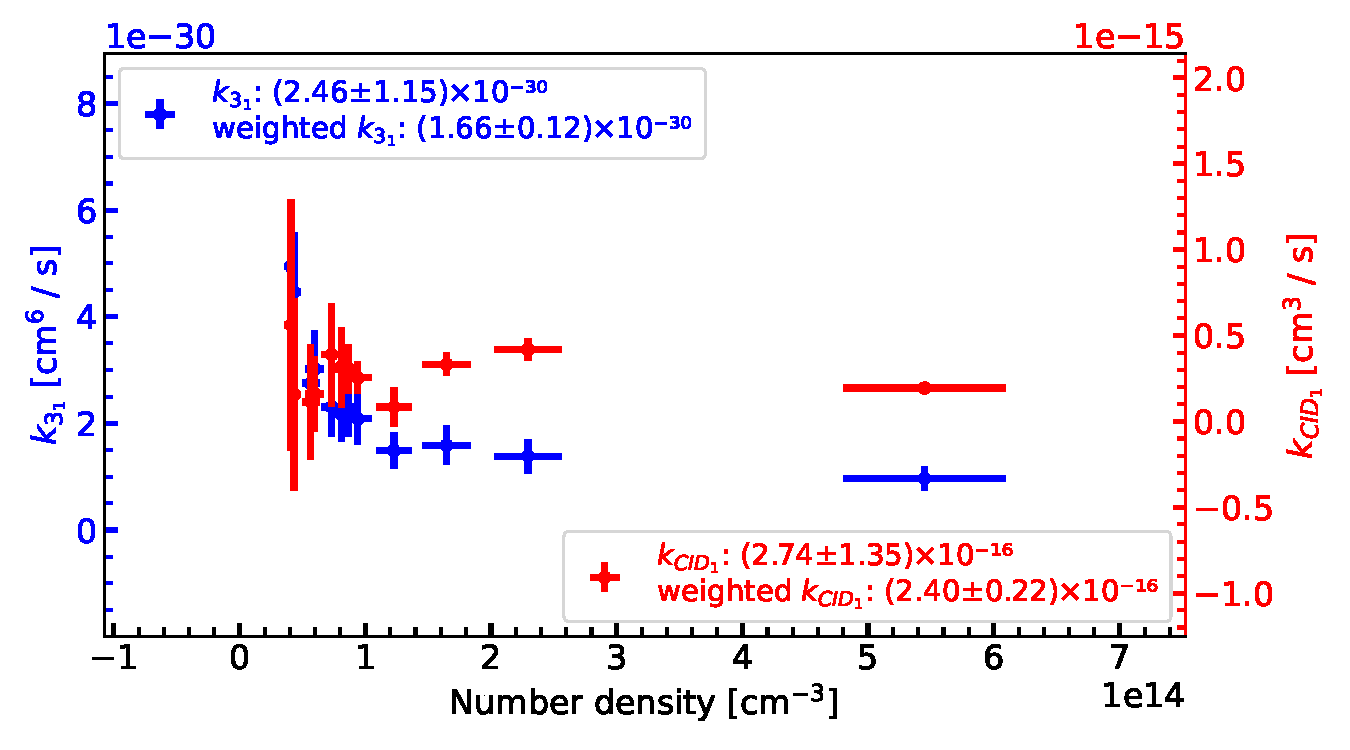
\includegraphics[width=1\textwidth]{figures/measurements/kinetics/functionOf_nHe/N+/off_10K_k3_kCID_1_as_functionOfnHe.pdf}}{}{\label{fig:off:10k-rate-constants:N+}}
    \hfill
    \end{adjustbox}
    \caption{
        N$^+$ + He reaction rate constants at $ (a) \& (b) \Rightarrow 4.8(3)$ K, $ (c) \& (d)\Rightarrow6.5(3)$ K, $ (e) \& (f)\Rightarrow8.4(3)$ K and $ (g) \& (h)\Rightarrow10.0(4)$ K: 
        The ternary association (\textcolor{blue}{$k_{3_1}$}) and collision-induced dissociation (\textcolor{red}{$k_{CID_1}$}) rate constants are plotted as a function of helium number density.
        (a, c, e, g) - represents: Effective binary rate constants are plotted as a function of number density to derive $k_{3_1}$ (ternary association) and $k_r$ (radiative) rate coefficients. 
        The solid line indicates the linear fit where the slope and intercept correspond to $k_3$ and $k_r$, respectively. 
        (b, d, f, h) corresponds to formation rate without $k_r$, the weighted average values are shown in the legend box (see Section \ref{subsec:rate-constants}).
    }
     \label{fig:rate-constants:N+}
\end{figure}